% !TeX spellcheck = en_US
\documentclass[a4paper,12pt]{article}

\usepackage{fullpage}
\usepackage{fourier}
\usepackage{amsmath}
\usepackage{color}
\usepackage{graphicx}
\usepackage{titlesec}

\titleformat{\subsection}[hang]{\large\bfseries}{\alph{subsection})\quad}{0pt}{}

\newcommand{\twodo}[1]{\textcolor{red}{\textbf{todo:} #1}}

\title{\textbf{Exercises for Image Processing 1}\\Problem Sheet 3}
\author{Axel Brand\\6145101 \and Nourhan Elfaramawy\\6517858 \and Konstantin M\"ollers\\6313136 \and Sibel Toprak\\6712316}

\begin{document}
	\maketitle
	
	\section{Perspective Transforms}
	
	\subsection{Straight Line Projection}
	
	A straight line in a 3D scene can be described by the following formula:
	
	\begin{align}\label{eqn:1} \vec{t} = \vec{p} + r \cdot \vec{d},\end{align}
	where $\vec{p}$ is a position vector and $\vec{d}$ is a direction vector. Every possible point on the line $\vec{t}$ can be reached by finding the appropriate $r$.
	
	Furthermore, we can split the equation~\ref{eqn:1} into its components:
	\begin{align}
		t_x &= p_x + r \cdot d_x \\
		t_y &= p_y + r \cdot d_y \\
		t_z &= p_z + r \cdot d_z.
	\end{align}
	
	If we now perform the projection, we obtain the following formulas:
	\begin{align}
		\label{eqn:2} t'_{x} &= t_x \cdot \frac{f}{t_z} \\
		\label{eqn:3}t'_{y} &= t_y \cdot \frac{f}{t_z}\\
		t'_{z} &= f.
	\end{align}
	
	From equations \ref{eqn:2} and \ref{eqn:3} we can conclude a straight line vector specification for a 2D scene:
	
	\begin{align}\label{eqn:4} \vec{s} = \vec{0} + \frac{f}{t_z} \cdot \binom{t_x}{t_y}.\end{align}
	
	Because we were able to construct a 2D straight line formula from any 3D one, we have shown that the obtained 2D projection stays a straight line. $\square$
	
	\subsection{Parallel Line Projection}
	
	In the case of \textbf{Orthographic projection}. Then all lines which are parallel in the real world are also parallel in the projected world.
	
	\textbf{Alternative Answer}:
	
	Parallel lines in space project perspectively onto lines that on extension intersect at a single point in the image plane called vanishing point or point at infinity. The vanishing point of a line depends on the orientation of the line and not on the position of the line. The vanishing point of any given line in space is located at the point in the image where a parallel line through the center of projection intersects the image plane.
	
By inserting into a Cartesian scene a set of parallel lines that are not parallel to any of the three axes of the scene, a new distinct vanishing point is created. Therefore, it is possible to have an infinite-point perspective if the scene being viewed is not a Cartesian scene but instead consists of infinite pairs of parallel lines, where each pair is not parallel to any other pair.

	
	\subsection{Sphere Projection}
	
	Given a sphere in the scene, we can visualize the set of points which connect the optical center of the camera to the edges of the visible hemisphere of the sphere as being a geometrical cone with the same radius and the top angle lying on the center. This cone is sliced by the image plane and rendered 2- dimensional exactly how the sphere is represented on the resulting picture.
So given a not null focal distance, a normal optical axis to the image plane and a sphere lying on a side of the image plane, the sphere will result in a circle in the image if its center point lies on the optical axis of the camera, thus the geometrical cone is then sliced by a plane parallel to its base, while in any other case the sphere will be an ellipse.


	
	Spheres are looking like ellipses in a 3D projection:
	
	\begin{figure}[h!]
		\centering
		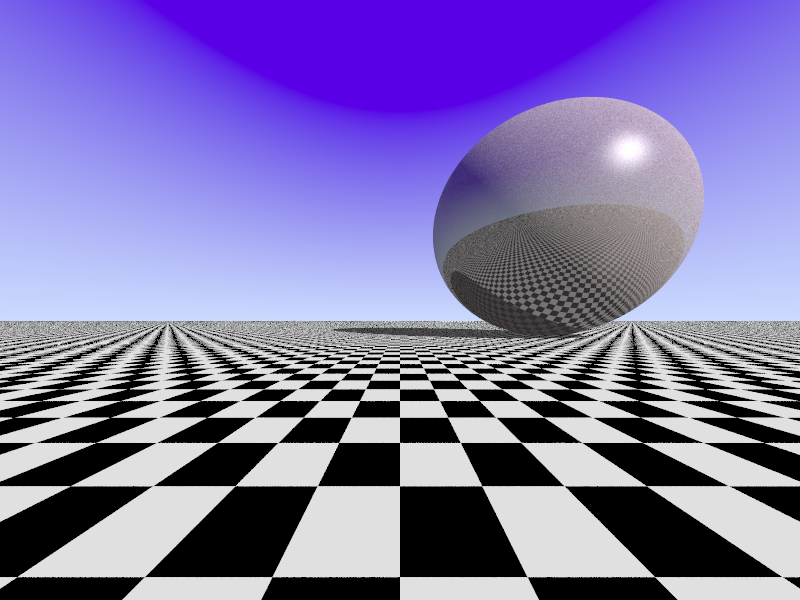
\includegraphics[width=0.7\textwidth]{E03.png}
		\caption{Sphere rendered with perspective projection in POV-Ray.}
	\end{figure}
	
	
\end{document}
